% !TeX program = xelatex
% IEEE 双栏会议格式研究计划。
\RequirePackage[T1]{fontenc}
\documentclass[conference]{IEEEtran}

% scheme=plain 保留 IEEEtran 的标题、章节和页面设置。
\usepackage[UTF8,scheme=plain,fontset=fandol]{ctex}
\setmainfont{TeX Gyre Termes}
\setsansfont{TeX Gyre Heros}
\setmonofont{TeX Gyre Cursor}
\setCJKmainfont{FandolSong-Regular.otf}[
    BoldFont=FandolSong-Bold.otf,
    ItalicFont=FandolKai-Regular.otf,
    BoldItalicFont=FandolKai-Regular.otf,
    SmallCapsFont=FandolSong-Regular.otf]
\usepackage{cite}
\usepackage{amsmath,amssymb}
\usepackage{booktabs}
\usepackage{graphicx}
\usepackage{balance}
\usepackage{xurl}
\usepackage[hidelinks]{hyperref}
\urlstyle{tt}
\hypersetup{pdfauthor={Yu Zhang}}
\renewcommand{\abstractname}{摘要}
\renewcommand{\IEEEkeywordsname}{关键词}
\renewcommand{\refname}{参考文献}

\title{C/C++ 漏洞检测评估研究计划\\基于独立函数与漏洞修复配对数据}
\author{
\IEEEauthorblockN{Yu Zhang}
\IEEEauthorblockA{ShanghaiTech University\\
Shanghai, China\\
\href{mailto:Zhangyu12026@shanghaitech.edu.cn}{Zhangyu12026@shanghaitech.edu.cn}}
}

\begin{document}
\maketitle

\begin{abstract}
本研究计划考察漏洞检测器识别单个漏洞函数，以及区分同一函数漏洞版本与对应修复版本的能力。研究从本地 SecVulEval 数据中构建两组互补的评估子集：第一组包含 200 条函数记录，其中 160 条标记为有漏洞、40 条标记为无漏洞，所选函数之间不存在数据集已标注的漏洞修复配对关系；第二组包含 200 对漏洞版本及其对应修复版本，共 400 条函数记录。配对严格依据原始数据的修复索引，两个子集在原始记录索引及“项目与提交”分组上相互隔离，合计包含 600 条不同的函数记录。本文阐明研究问题、抽样约束、可复现信息及有效性限制，为后续开展函数级检测与修复差异辨识评估提供基础。实验方法、实验模型和实验结果将在后续研究中补充。
\end{abstract}

\begin{IEEEkeywords}
漏洞检测，C/C++，评估数据集，配对评估，可复现性
\end{IEEEkeywords}

\section{研究背景与动机}
自动化漏洞检测旨在帮助开发者识别源代码中的安全缺陷。评估不仅需要考察检测器能否识别有漏洞函数、减少对无漏洞函数的误报，还需要回答另一个问题：当同一函数经过漏洞修复后，检测器能否相应改变判断。因此，单个函数与明确关联的漏洞修复版本对，可以作为两类互补的评估单元。

正式发表于 AIware 2026 的 SecVulEval 提供包含语句级变更标注和上下文信息的 C/C++ 函数样本~\cite{ahmed2026secvuleval}。PrimeVul 强调数据质量、污染控制，以及通过漏洞函数及其补丁开展评估~\cite{ding2025primevul}。这些工作为结合函数级分类与安全相关变更敏感性开展研究提供了依据。本研究在本地 SecVulEval 快照上设计规模明确、可复现的评估子集，现阶段的重点是评估数据设计。

在独立函数子集中，检测器需要评估未同时包含已标注修复对应版本的函数；在配对子集中，则可以考察其对同一函数漏洞版本和修复版本的判断是否与标签一致。分别观察这两种情形，有助于揭示单一总体结果可能掩盖的行为差异。本文中的“独立”指抽样与修复关联约束，不表示样本在统计意义上完全独立。

\section{研究目标与研究问题}
本研究旨在建立可追溯的评估基础，区分函数级漏洞识别能力与漏洞修复差异辨识能力，重点回答以下问题：
\begin{enumerate}
    \item \textbf{RQ1：函数级检测。} 在包含 160 条有漏洞函数和 40 条无漏洞函数的独立子集中，检测器能够在多大程度上正确识别漏洞并排除无漏洞样本？
    \item \textbf{RQ2：漏洞修复差异辨识。} 对于同一函数的两个版本，检测器能否识别漏洞版本，并将对应修复版本判定为数据集标签所定义的无漏洞版本？
    \item \textbf{RQ3：两类子集的互补性。} 面向独立函数与存在修复关联的函数版本，检测器会表现出哪些不同的判断行为？
\end{enumerate}

两个子集定位为评估资源，尚未被定义为训练集与测试集。若后续需要训练、调参或开发数据，应另行明确其来源和隔离方式。检测器有效性的结论，将在实验方案和模型确定并完成评估后给出。

\section{数据集构建方案}
\subsection{数据来源与记录校验}
数据源为本地 \texttt{SecVulEval.xlsx} 的 \texttt{train} 工作表，对应 SecVulEval 基准及其数据发布~\cite{ahmed2026secvuleval,secvulevaldata}。本地工作簿包含 25,440 条函数记录，其中 10,998 条标记为有漏洞，14,442 条标记为无漏洞。这些数量描述的是本研究实际使用的本地数据文件。

构建脚本检查原始索引、标签、必要文本字段及序列化列表字段。由于 7 条记录的 \texttt{changed\_statements} 无法解析，实际保留 25,433 条可用记录，并在 JSON 元数据中保存排除索引及原因。缺失或已排除的修复目标不能构成有效配对；去除首尾空白后函数正文相同的版本对也予以排除。经过当前校验，可用于抽样的候选配对共 10,004 对。

\begin{figure*}[t]
\centering
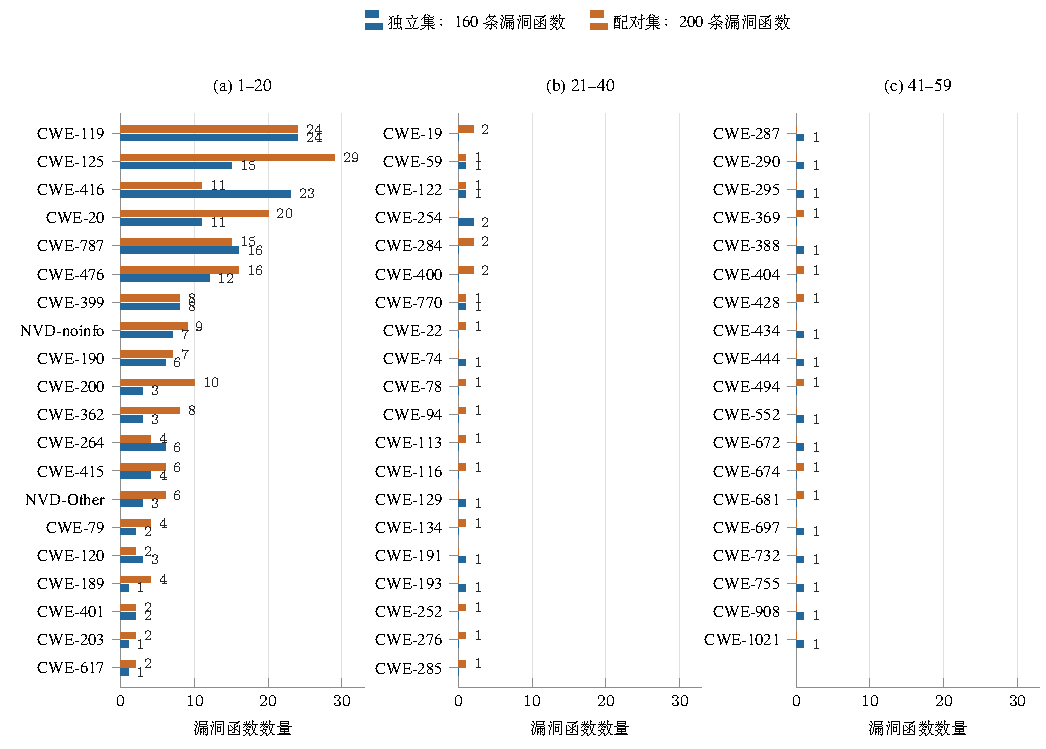
\includegraphics[width=\textwidth]{figures/cwe_distribution_zh.pdf}
\caption{按规范化 CWE 标签统计的漏洞函数数量。图中完整展示 57 种数字 CWE 类型及两类 NVD 占位标记，按两组计数之和从高到低排列，三个面板采用相同横轴刻度。NVD-noinfo 和 NVD-Other 分别表示 NVD-CWE-noinfo 与 NVD-CWE-Other，是元数据标记而非具体漏洞类型。零计数柱不标注数值；每对漏洞修复版本仅计入漏洞版本一次。}
\label{fig:cwe-distribution}
\end{figure*}

\subsection{子集 A：独立函数集}
将独立函数集表示为
\begin{equation}
\mathcal{D}_{\mathrm{ind}}=\{(x_i,y_i)\}_{i=1}^{200},
\qquad y_i\in\{0,1\},
\end{equation}
其中 $x_i$ 为函数记录，$y_i=1$ 表示有漏洞标签。该集合严格包含 160 条有漏洞函数和 40 条无漏洞函数，并满足：
\begin{enumerate}
    \item 每个 \texttt{(project, commit\_id)} 分组最多选取一条函数记录。
    \item 任一入选漏洞函数在数据中标注的修复版本，不同时出现在该集合中。
    \item 40 条无漏洞函数均不是原始工作簿中任意漏洞记录通过修复索引指向的修复版本。
\end{enumerate}
这些条件实现了所选样本之间不存在已标注修复配对关系的设计目标。约束针对数据集记录的关联，不构成对上游完整 Git 历史中所有可能关系的证明。

\subsection{子集 B：漏洞修复配对集}
将配对集表示为
\begin{equation}
\mathcal{D}_{\mathrm{pair}}=
\{(x_j^{v},x_j^{f})\}_{j=1}^{200},
\end{equation}
其中 $x_j^{v}$ 为标记有漏洞的版本，$x_j^{f}$ 为其对应修复且标记无漏洞的版本。配对必须满足原始索引关联：
\begin{equation}
\texttt{fixed\_func\_idx}(x_j^{v})=\texttt{idx}(x_j^{f}).
\end{equation}
此外，两个版本的项目、提交标识、文件路径及函数名必须一致，且去除首尾空白后的函数正文必须不同。共享提交标识用于数据标注的分组；版本配对由 \texttt{fixed\_func\_idx} 确定，不通过不同提交标识推测先后顺序。每个项目与提交分组最多选择一对。

因此，该集合包含 200 对、共 400 条函数记录。评估目标是同时正确判断漏洞版本与修复版本。两个版本分别输入还是联合输入，属于后续实验方案需要确定的问题。

\begin{table}[t]
\caption{两类评估子集的组成}
\label{tab:composition}
\centering
\begin{tabular}{@{}lcrrr@{}}
\toprule
子集 & 评估单元 & 有漏洞 & 无漏洞 & 函数总数\\
\midrule
$\mathcal{D}_{\mathrm{ind}}$ & 200 条函数 & 160 & 40 & 200\\
$\mathcal{D}_{\mathrm{pair}}$ & 200 对版本 & 200 & 200 & 400\\
\bottomrule
\end{tabular}
\end{table}

\subsection{抽样顺序与集合隔离}
抽样使用局部随机数生成器 \texttt{random.Random(42)}。首先打乱候选配对并选取 200 对；随后在排除已使用项目与提交分组的基础上，依次选择 160 条有漏洞函数和 40 条符合条件的无漏洞函数，导出前再次打乱独立函数记录。当前没有额外设置项目、CWE 类型或代码长度配额。

设 $I(\mathcal{D})$ 为集合中的原始记录索引，$G(\mathcal{D})$ 为项目与提交分组，则构建过程保证：
\begin{align}
I(\mathcal{D}_{\mathrm{ind}})\cap I(\mathcal{D}_{\mathrm{pair}})&=\varnothing,\\
G(\mathcal{D}_{\mathrm{ind}})\cap G(\mathcal{D}_{\mathrm{pair}})&=\varnothing.
\end{align}
两个集合合计包含 600 条不同的原始记录。相同项目仍可通过不同提交出现在两个集合中，因此当前设计不属于项目完全隔离的划分。

\subsection{数据产物与可复现性}
独立函数保存在 \path{independent_200.json} 的 \texttt{samples} 数组中；配对记录保存在 \path{vulnerable_fixed_200_pairs.json} 的 \texttt{pairs} 数组中，每对包含 \texttt{pair\_id}、\texttt{vulnerable} 和 \texttt{fixed}。每条记录保留全部 16 个原始字段、完整函数正文与源索引。序列化列表转换为 JSON 数组，\texttt{context} 保留原始字符串且不执行其内容。

构建脚本 \path{build_datasets.py} 已在 Conda \texttt{pap} 环境中运行，所用版本为 Python 3.12.16、\texttt{openpyxl} 3.1.5 和 \texttt{et\_xmlfile} 2.0.0。元数据记录随机种子、源文件 SHA-256、排除项及抽样约束。已将导出的记录与工作簿逐字段核对，并验证种子 42 能复现同样的输出。这些检查属于数据构建与序列化校验，不属于漏洞检测实验结果。

\subsection{CWE 漏洞类型分布}
图~\ref{fig:cwe-distribution} 展示独立集的 160 条漏洞函数与配对集的 200 条漏洞版本的通用弱点枚举（Common Weakness Enumeration，CWE）数量分布，不计入 40 条独立集负样本和 200 条修复版本。描述性统计时，将 \texttt{CWE-125CWE-787} 等连写标签拆分为独立 CWE 编号，并在每个函数内去重；原始 JSON 文件保持不变。两组漏洞样本各覆盖 39 种明确的数字 CWE 类型，合并后共 57 种。计入两类 NVD 占位标记后，标签归属总数分别为 173 和 213；由于部分函数具有多个 CWE 标签，归属总数超过漏洞函数数量。

\balance
\section{研究范围与有效性限制}
独立函数集采用人为设定的 80\% 有漏洞比例，该比例不能解释为真实软件中的漏洞发生率；配对集则因配对要求而具有平衡标签。因此，若后续汇总两个子集的结果，需要明确其样本构成与解释范围。

本研究继承数据源的标签和修复关联。无漏洞标签，或针对已标注问题的修复，不证明函数不存在其他安全缺陷。项目与提交隔离能够控制一类记录重叠，但不能保证消除相似代码、共同漏洞家族或模型预训练污染。当前设计也不支持项目完全隔离或时间外推的泛化结论。

样本规模较小，且没有按 CWE 分层，因而覆盖范围有限。同一配对内的两个版本是相关观测，不能将其中 400 条函数视为 400 个互不相关的评估单元。标签、修复索引、提交说明、CVE 及变更标注用于保留可追溯性；未来实验必须明确哪些字段可作为模型输入，避免泄露待预测答案。失败处理及额外开发集的设计也有待确定。

\section{预期贡献}
本研究拟提供可复现的双子集评估资源，明确区分单函数检测与漏洞修复差异辨识，并为分析两种评估情形下的行为差异建立可追溯基础。目前已有数据构建产物，尚未形成关于实验方法、模型优劣或性能的结论。

\section{实验方法}
\label{sec:methods}
% 按要求暂留空白。后续补充实验流程、输入字段、评价指标、
% 失败处理及统计分析，不在当前版本预设实验方案。

\section{实验模型}
\label{sec:models}
% 按要求暂留空白。后续补充模型名称、版本及配置。

\section{实验结果}
\label{sec:results}
% 按要求暂留空白。完成实验后填写实测结果及分析。

\bibliographystyle{IEEEtran}
\bibliography{references}
\end{document}
